\documentclass[10pt]{article}
\usepackage{amsmath}
\usepackage{amsfonts}
\usepackage{graphicx}
%\usepackage{epstopdf}
\usepackage{hyperref}
\usepackage[left=.9in,right=.9in,top=.7in,bottom=.7in]{geometry}
%\usepackage[left=1.1in,right=1.1in,top=.7in,bottom=.7in]{geometry}
\usepackage{multirow}
\usepackage{verbatim}
\usepackage{fancyhdr}
\usepackage[small,compact]{titlesec} 
\usepackage{color}
\usepackage{ulem}
%\usepackage[screen,nopanel,gray]{pdfscreen}
%\screensize{4in}{5.33in}
%\margins{0.75in}{0.75in}{0.75in}{0.75in}


%\usepackage{pxfonts}
%\usepackage{isomath}
\usepackage{mathpazo}
%\usepackage{arev} %     (Arev/Vera Sans)
%\usepackage{eulervm} %_   (Euler Math)
%\usepackage{fixmath} %  (Computer Modern)
%\usepackage{hvmath} %_   (HV-Math/Helvetica)
%\usepackage{tmmath} %_   (TM-Math/Times)
%\usepackage{cmbright}
%\usepackage{ccfonts} \usepackage[T1]{fontenc}
%\usepackage[garamond]{mathdesign}

\newcommand{\argmax}{\operatornamewithlimits{arg\,max}}
\newcommand{\argmin}{\operatornamewithlimits{arg\,min}}
\newcommand{\myTable}[1]{\begin{table}[b]\caption{#1}
    \begin{minipage}{\linewidth} \begin{center}}
\newcommand{\myTableEnd}{\end{center}\end{minipage}\end{table}}

\def\inprobLOW{\rightarrow_p}
\def\inprobHIGH{\,{\buildrel p \over \rightarrow}\,} 
\def\inprob{\,{\inprobHIGH}\,} 
\def\indist{\,{\buildrel d \over \rightarrow}\,} 

\newtheorem{theorem}{Theorem}

%\pagestyle{fancy}
\renewcommand{\sectionmark}[1]{\markright{#1}{}}
 
%\fancyhead[LE,LO]{\thepage}
%\fancyhead[CE,CO]{\rightmark}
%\fancyfoot[C]{}

\title{Economics 526 - Mathematics for Economists}
\date{Term 1, 2012}
\author{Paul Schrimpf}

\makeatletter
\renewcommand{\@maketitle}{
  \null
  \begin{center}%
    {\large \textbf{\@title} \par \normalsize \@date \par \@author}%
  \end{center}%
  \par} 
\makeatother

\begin{document}

\maketitle

This is a course of mathematics for students in our Economics MA
program. It covers powerful mathematical tools that often appear
in the modern economic literature. It is essential for the students'
success in other courses to master the materials taught in this
course.

Yawen Liang (neway.liang@gmail.com) and Stephen Zhengfei Yu
(yuzhengfei@gmail.com) are the course TA's.  Information about the
course will be sent via e-mail.  Lecture notes are posted at
\url{http://faculty.arts.ubc.ca/pschrimpf/526/526.html}. Currently,
these notes are from last year. The notes will be updated throughout
the term. Problem sets, solutions, and grades will be posted on the
course's \url{http://vista.ubc.ca} page.

 My email is
\href{mailto:schrimp@mail.ubc.ca}{schrimpf@mail.ubc.ca}, and my office
phone number is 604-822-5360.

\section{Schedule}
\begin{tabular}{l c c l}
  \hline 
  & \textbf{Day(s)} & \textbf{Time} & \textbf{Location} \\
  Lecture & Monday \& Wednesday & 2:00pm-4:00pm & IKBLC 261  
  \\
  Tutorial & Wednesday & 11:00am-12:30pm & SWNG 407 \\  
  \\
  Office hours \\
  \; Paul & Monday & 10:00am-11:00am & Buchanan Tower 926 \\
  \; Yawen & TBA & & \\ 
  \; Stephen & TBA & & \\ \hline
  Exams \\
  \; Midterm & Wednesday, October 3rd & 2:00pm-4:00pm & IKBLC 261 \\
  \; Final & Wednesday, November 14th & 2:00pm-4:00pm & IKBLC 261 \\
  No class \\
  \; Thanksgiving & Monday, October 8th \\
  \; Out of town & Monday, November 5th \\  
  \\ \hline 
\end{tabular} \\
Office hours are subject to change. Any changes in office hours will
be posted on the course web page. If you cannot come to my office
hours, feel free to drop by anytime or email me to schedule an
appointment.  I will be out of town October 4th-7th, October
26th-28th, and from November 5th until 12:30pm on November 7th. We will
plan on having lecture on Wednesday November 7th, but it may start
late or be canceled if my flight arrives late. 

\section{Course Work}

The course work will consist of a series of problem sets and two
exams. 

\subsection{Problem Sets}
Problem sets will be due approximately weekly.  Students should solve
each problem set and turn in their work by the specified due
date. Also, students should study the solution to each problem set
carefully, regardless of their performances in the problem
set. Students may work together on problem sets, but each student
should write their own solutions.

\subsection{Exams}
Two in-class exams will be given on October 3rd and November 14th. If
a student misses the first exam due to an objectively verifiable,
unavoidable emergency situation, the student's grade will be
determined by setting his first exam's grade equal to his second
exam's grade. If a student misses the first exam for any other
reasons, the student receives zero points for the first exam.

\subsection{Grading}
The course grade weights the problem sets by 0.15, the First exam by
0.40 and the second exam by 0.45. If a student finds an error in the
grading of a problem set or exam, the student should contact the
teaching assistants (for problem sets) or me (for an exam) within one
week of the day the graded problem sets or exams were made
available. We will then regrade the entire problem set or exam, and
your total score may increase or decrease as a result.  The
distribution of grades in this course for the past five years is shown
below.
\href{http://www.arts.ubc.ca/faculty-amp-staff/resources/courses-and-grading/grading-guidelines.html}
{The Faculty of Arts grading guidelines} recommend that 5-25\% of the
class receive A's (80-100) and not more than 75\% receive A's or B's
(68-79). Grades may be scaled up to meet these guidelines and/or match
the historical distribution of grades, but they will not be scaled
down.

\begin{centering}
  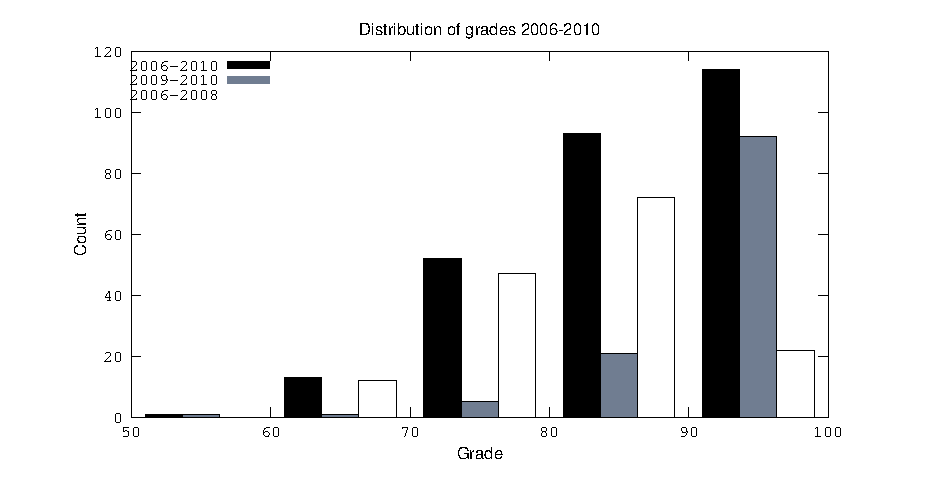
\includegraphics[width=0.8\linewidth]{526gradeDist}
\end{centering}

\section{Textbook}

There is no required textbook for this course, but buying one is
recommended.  The notes are largely based on \textit{Mathematics for
  Economists} by Simon and Blume. Compared to the notes, Simon and
Blume place less emphasis on proofs and more emphasis on examples and
exercises. Since the notes are based on it, Simon and Blume is
probably the best book to buy if you want something just to clarify
lectures and help for problem sets. However, Simon and Blume is not
especially nice to read. It doesn't have enough economic motivation
and examples to appeal to practical-minded readers, and it isn't
rigorous or elegant enough to please mathematicians.

\textit{Fundamental Methods of Mathematical Economics} by Chiang and
Wainwright is a good choice if you have little background in
mathematics and/or found the review exercises difficult. Chiang and
Wainwright is easier to read and has more economic motivation and
examples than Simon and Blume. However, Chiang and Wainwright does not
contain any proofs. 

\textit{Foundations of Mathematical Economics} by Carter is an excellent
book, but is more difficult than the previous two. It contains many
proofs and can be quite abstract. However, it does do a good job of
motivating everything with economic examples. I recommend it if you
have a solid mathematics background or plan to apply to continue
studying economics after the Master's program. Carter is the only of
the three books that is sophisticated enough to remain a useful
reference throughout a PhD program and beyond.

All three books are available in affordable paperback
editions. Unfortunately, the UBC bookstore was unable to order
paperback editions, so you may want to order your book(s) elsewhere. 

\section{Course Outline}

The topics of the course are outlined below. The corresponding part of
Simon and Blume and the projected number of lectures of each topic are
indicated in parentheses.
\begin{enumerate}
\item Sets, Numbers, and Proofs (Appendix A1; 0.5 lectures)
\item Linear Algebra
  \begin{enumerate}
  \item Systems of Linear Equations (Chapters 6-7; 1 lecture)
  \item Matrix Algebra (Chapters 8-9, 26; 1.5 lecture)
  \item Euclidean Spaces as Linear Spaces (Chapters 10-11, 27; 2
    lectures)
  \item Eigenvalues, Eigenvectors, and Definite Matrices (Chapter 23,
    16; 1 lecture)
  \end{enumerate}
\item Calculus of Several Variables
  \begin{enumerate}
  \item Topology of the Euclidean Spaces (Chapter 12, 29 (up to
    Section 29.3); 1 lecture) 1 
  \item Functions (Chapter 13; 1.5 lecture)
  \item Differential Calculus (Chapters 14, 30, 1 lecture)
  \item Contraction Principle, Inverse Function Theorem, and Implicit
    Function Theorem (Chapter 15; 0.5 lecture)
  \end{enumerate}
\item Optimization
  \begin{enumerate}
  \item Unconstrained Optimization (Chapter 17; 0.5 lectures)
  \item Constrained Optimization (Chapters 18-19; 1.5 lectures)
  \item Homogeneous and Homothetic Functions (Chapter 20; 1 lectures)
  \item Concave and Quasiconcave Functions (Chapter 21; 1 lecture)
  \end{enumerate}
\item Dynamic programming and Optimal Control (1 lecture) 
  % guido and ivan's notes on ocw, daron's book chs 6, 7 , 16
\item Comparative statics without differentiability: Supermodularity
  and Topkis's theorem (1 lecture)
  \begin{itemize}
  \item Reference: Amir, Rabah (2005). ``Supermodularity and
    Complementarity in Economics: An Elementary Survey,''
    \textit{Southern Economic Journal}. 71(3):
    636-660. \url{http://www.jstor.org/stable/20062066}
  \end{itemize}
\end{enumerate}

\end{document}

